\section{Konzept der Ereignisverarbeitung}\label{sec:Ereignisverarbeitung}
In der realen Welt ist eine Wechselwirkung aller Geschehnisse mit einer Vielzahl von divergenten, meist nicht-deterministisch eintretenden Ereignissen zu beobachten, als Konsequenz folgt eine signifikante Beeinflussung auf den Fortgang der Geschehnisse.
\cite{Grauer.2010}
Dieser Tatbestand findet sich auch in den Abläufen und Geschäftsprozessen in Unternehmen wieder.
Ein Unternehmen ist demzufolge gezwungen, auf diese Ereignisse angemessen und möglichst zeitnah zu reagieren – die Unternehmen operieren demnach ereignisgesteuert. 
\cite{Schaaf.2015}
Mit dem Konzept der Ereignisverarbeitung rücken Ereignisse als zentraler Leitgedanke einer Orientierung an Ereignissen in den Fokus der Gestaltung von Geschäftsprozessen, indem Ereignisse als Baustein der Softwarearchitektur und der Geschäftslogik in den Mittelpunkt der Betrachtung rücken. 
\cite{Bruns.2010}

Die resultierenden ereignisgesteuerten Unternehmensanwendungen ermöglichen eine praxisnahe Darstellung der dynamischen Geschäftsprozesse eines Unternehmens. 
Das Ziel ist es dadurch die Agilität, Reaktionsfähigkeit und Echtzeitfähigkeit der Geschäftsprozesse eines Unternehmens zu erhöhen. 
In der Praxis hat eine derartige Ereignisorientierung in Unternehmensanwendungen bereits breiten Zuspruch gefunden. 
\cite{Bruns.2015}
In diesem Kontext beruhen ereignisgesteuerte Architekturen, englisch \ac{EDA}, auf einem ereignisgesteuerten Prinzip, bei dem eine lose Kopplung zwischen den beteiligten Komponenten eines Informationssystems vorgesehen ist.  
In ihrer reinen Ausprägung kommunizieren diese Komponenten ausschließlich mittels sogenannter Ereignisbenachrichtigungen, englisch \textit{Event Messages}, miteinander.
Abbildung \ref{fig:Grundschritte von ereignisgesteuerten Architekturen} illustriert den Ablauf der Grundschritte ereignisgesteuerter Architekturen, deren Charakteristika nachfolgend erläutert werden.
\cite{Schaaf.2015}

\begin{figure}[H]
	\centering 
    \begin{tikzpicture}
        \fill[even odd rule, white] circle (1.5);
    
       \node at (0,0) [
          font  = \sffamily\Large\bfseries\color{black!85},
          align = center
       ]{
          \acs{EDA}
       };
       \arcarrow{197}{ 96}{Erkennen}
       \arcarrow{ 89}{-17}{Verarbeiten}
       \arcarrow{199}{341}{Reagieren}
    \end{tikzpicture}
    \caption[Grundschritte von ereignisgesteuerten Architekturen]
    {Grundschritte von ereignisgesteuerten Architekturen \protect\footnotemark}
    \label{fig:Grundschritte von ereignisgesteuerten Architekturen}
\end{figure}
\footnotetext{in Anlehnung an \citeauthor{Bruns.2010} \citeyear{Bruns.2010} \cite{Bruns.2010} }

Demnach besteht eine zentrale Charakteristik von ereignisgesteuerten Architekturen aus der Komposition von drei Grundschritten: \textit{Erkennen, Verarbeiten und Reagieren von oder auf Ereignisse.}

\paragraph{Erkennen} 
Das Auftreten von relevanten Informationen und Sachverhalten in  den Geschäftsprozessen ist der Ausgangspunkt für die Erkennung von Ereignissen.
Diese Informationen und Sachverhalte werden analysiert, als Ereignisse klassifiziert und spiegeln einen spezifizierten Ausschnitt des Zustands eines Geschäftsprozesses wieder. 
Für registrierte Ereignisse wird ein entsprechendes Ereignisobjekt generiert.
Entscheidend für ereignisgesteuerte Informationssysteme ist, dass die Ereignisse unmittelbar zum Zeitpunkt ihres Auftretens erkannt werden und nicht zeitverzögert.
\cite{Bruns.2010}

\paragraph{Verarbeiten}
Im Verarbeitungsschritt werden die erkannten Ereignisse, die aus unterschiedlichen Ereignisquellen stammen können, analysiert. Bei der Analyse werden Ereignisse zu Einheiten aggregiert, mit anderen Ereignissen verknüft, generalisiert, aufgeteilt oder aber auch als irrelevant eingestuft. 
Gesucht werden Paradigmen in den gesammelten Ereignissen, die bestimmte Beziehungen und Abhängigkeiten zwischen den Ereignissen ausdrücken.
\cite{Hedtstuck.2017}

\paragraph{Reagieren}
Aufgrund von analysierten Mustern, die im Fluss der eingetretenen Ereignisse erkannt wurden, können vielfältige Arten von Reaktionen zeitnah veranlasst werden. 
Die Reaktionen, die angestrebt werden, charkterisieren sich durch Aktualität und Individualität, wie etwa die unmittelbare Übergabe der Ereignisse an Anwendungssysteme, das Senden von Benachrichtigungen, der Aufruf von Funktionen in Form von digitalen Diensten, das Auslösen eines Geschäftsprozesses oder die Initiierung von manuellen Aktivitäten durch menschliche Benutzer, aber auch die Generierung neuer Ereignisse ist eine legitime Reaktion.
\cite{Bruns.2010}

In der Realität existieren allerdings kaum Geschäftsprozesse, bei denen eine ausschließliche Kommunikation mithilfe von Ereignissen und alleinig im Rahmen der beschriebenen Grundschritte einer \ac{EDA} erfolgen, weshalb auch Anwendungen mit teilweiser Ereignisverarbeitung und partieller Anwendung dieser Grundschritte die Umsetzung einer ereignisgesteuerten Architektur zugeschrieben.
\cite{Etzion.2011}
Die \ac{SOA}-Architektur beinhaltet, wie in Abschnitt \ref{sec:Automatisierung} beschrieben, die Konzepte, die notwendig sind, um Echtzeit-Anwendungssysteme zu ermöglichen und die Unterstützung der Dynamik ereignisgesteuerter Geschäftsprozesse zur selben Zeit zu gewährleisten, nicht vollständig.
Eine \ac{SOA} ohne Ereignisverarbeitung ist folglich nicht in der Lage, den aktuellen Zustand von Aktivitäten zu erkennen, da hierzu in Echtzeit temporale und kausale Verbindungen zwischen Geschäftsprozessen und Aktivitäten identifiziert und analysiert werden müssen. 
Eine \ac{EDA} kann als Maßnahme auch eine \ac{SOA} komplementieren, zumal beide Konzepte grundsätzlich modulare und verteilte Informationssysteme mit loser Kopplung unterstützen, um die Vorteile beider Architekturen im Kollektiv zu nutzen. 
Für eine derartige Kombination von \ac{SOA} und \ac{EDA} wird häufig die Bezeichnung Event-Driven SOA genutzt.
In dieser Ausprägung können Ereignisse den Aufruf von digitalen Diensten auslösen, woraufhin im Verlauf, deren Ausführung weitere Ereignisse generiert werden, die parallel von einem Ereignisverarbeitungsdienst analysiert und verarbeitet werden. 
\cite{Bruns.2010}

Im Zusammenhang mit der Ereignisverarbeitung in Unternehmensanwendungen wird der Begriff Echtzeit, englisch real-time, häufig verwendet, um die Aktualität von verarbeiteten Ereignissen zu hervorzuheben.
\cite{Bruns.2015}
Echtzeit wird jedoch nicht im Sinne der Informatik verstanden, wonach für jede Funktion die exakte Einhaltung einer restriktiv vorgeschriebenen Antwortzeit erforderlich ist, um die Gegenwartsbezogenheit und Vorhersagbarkeit von Informationssystemen sicherzustellen.
Vielmehr dominiert ein betriebswirtschaftliches Verständnis, das darauf Bedacht ist, in allen relevanten Informationssystemen aktuelle Informationen bereitzustellen, ohne spezifizierte Leistungskennzahlen zur Erfüllung von Echtzeit zu formulieren.
\cite{Worn.2005}
Unter Echtzeit versteht man aus dieser Sicht daher die möglichst zeitnahe Verfügbarkeit, Transparenz und Nutzbarkeit von Informationen ohne unnötige Zeitverzögerung.
Eingehende Ereignisse werden somit im Rahmen der Ereignisverarbeitung analysiert, sobald sie auftreten, um geeignete Reaktionen in Echtzeit auslösen zu können.
\cite{Grauer.2010}

\subsection{Merkmale und Kriterien}
Die \ac{EDA} wird, wie schon erwähnt, im Wesentlichen durch die drei Grundschritte Erkennen, Verarbeiten und Reagieren charakterisiert, woraus sich drei logische architektonische Schichten für eine Ereignisverarbeitung ergeben: Ereignisquellen, Ereignisverarbeitung und Ereignisbehandlung. Das
Zusammenspiel dieser drei Schichten wird  in Abbildung \ref{fig:Grundlegender architektonischer Entwurf einer EDA} veranschaulicht.

\begin{figure}[H]
	\centering 
    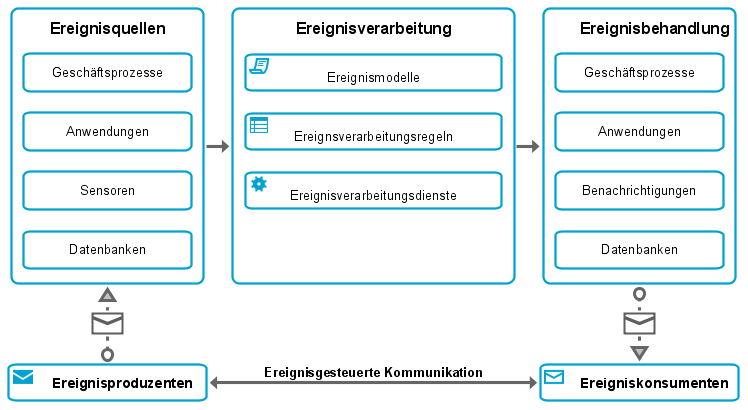
\includegraphics[width=\textwidth]{img/Ereignisverarbitungablauf.png}	
    \caption[Grundlegender architektonischer Entwurf einer EDA]
    {Grundlegender architektonischer Entwurf einer EDA}
    \label{fig:Grundlegender architektonischer Entwurf einer EDA}
\end{figure}
\footnotetext{in Anlehnung an \citeauthor{Metz.2014} \citeyear{Metz.2014} \cite{Metz.2014} }

\todo{abbildung erkären}

\todo{Formulierung der Ereignisverarbeitungsregeln}

\missingfigure{Kriterien für Funktionalitäten der Ereignisverarbeitung}

\subsection{Bewertung von Funktionalitäten der Ereignisverarbeitung}

\todo{Referenzieren auf \cite{Vidackovic.2010}}

\missingfigure{Tabelle  Bewertung von Funktionalitäten der Ereignisverarbeitung}

